\section{Template-Based Geometry Generation}

\todo[inline]{improve the mainly placeholder text, use the things we agreed upon with RF}

\subsection{Gmsh Template Files}

The geometry generation process relies on predefined Gmsh template files. These templates serve as flexible blueprints for creating a variety of geometries, with key parameters such as dimensions, resolution, and specific geometric features being dynamically filled based on the optimization parameters. The template files are structured to allow for easy modification, where placeholders represent variable values that are substituted programmatically during the optimization process.

% [Optional Figure suggestion: A snippet of a Gmsh template file, showing the placeholders and how they are replaced with actual values.]

Each Gmsh template is parameterized to accommodate variations in geometry. For example, the templates can define features such as the dimensions of the extracardiac conduit, pulmonary artery, or vena cava superior. Parameters such as the rotation angle or the mesh density are key elements that allow flexibility in the final geometry generated.

\subsection{Parameterization}

The optimization parameters dictate how the geometry templates are modified. Each parameter maps to a placeholder within the Gmsh file, which is replaced by the actual value provided during the optimization. This process ensures that each geometry is tailored precisely to the current set of optimization requirements.

One of the main challenges during parameterization is ensuring consistency across different geometries. This involves making sure that the parameters result in valid geometries that meet the required constraints for numerical simulations. Additionally, the range of allowable parameter values must be carefully managed to avoid issues such as mesh inconsistencies or geometry deformations.

\subsection{Example Workflow}

To illustrate the process, consider the generation of an extracardiac conduit. The Gmsh template defines the conduit using several geometric points, splines, and surfaces. The optimization parameters, such as the conduit diameter and length, are substituted into the template at predefined positions. Once the template is modified, Gmsh generates a 3D mesh of the conduit, which can then be further processed.

\begin{lstlisting}[language=C++]
	...
	// Define points along the axis of the upper cylinder
	Point(101) = {0.0, 0.0, LOWER_LENGTH + UPPER_LENGTH, h};
	Point(102) = {0.0, 0.0, LOWER_LENGTH, h};
	
	// Create line and wire for upper cylinder extrusion
	Line(101) = {102, 101};
	Wire(102) = {101};
	
	// Disk representing the base of the upper cylinder
	Disk(101) = {0.0, 0.0, LOWER_LENGTH + UPPER_LENGTH, UPPER_RADIUS};
	
	// Extrude the surface to form the second cylinder volume
	Extrude { Surface{101}; } Using Wire {102}
	...
\end{lstlisting}


\begin{figure}[H]
	\centering
	\vspace{6mm}
	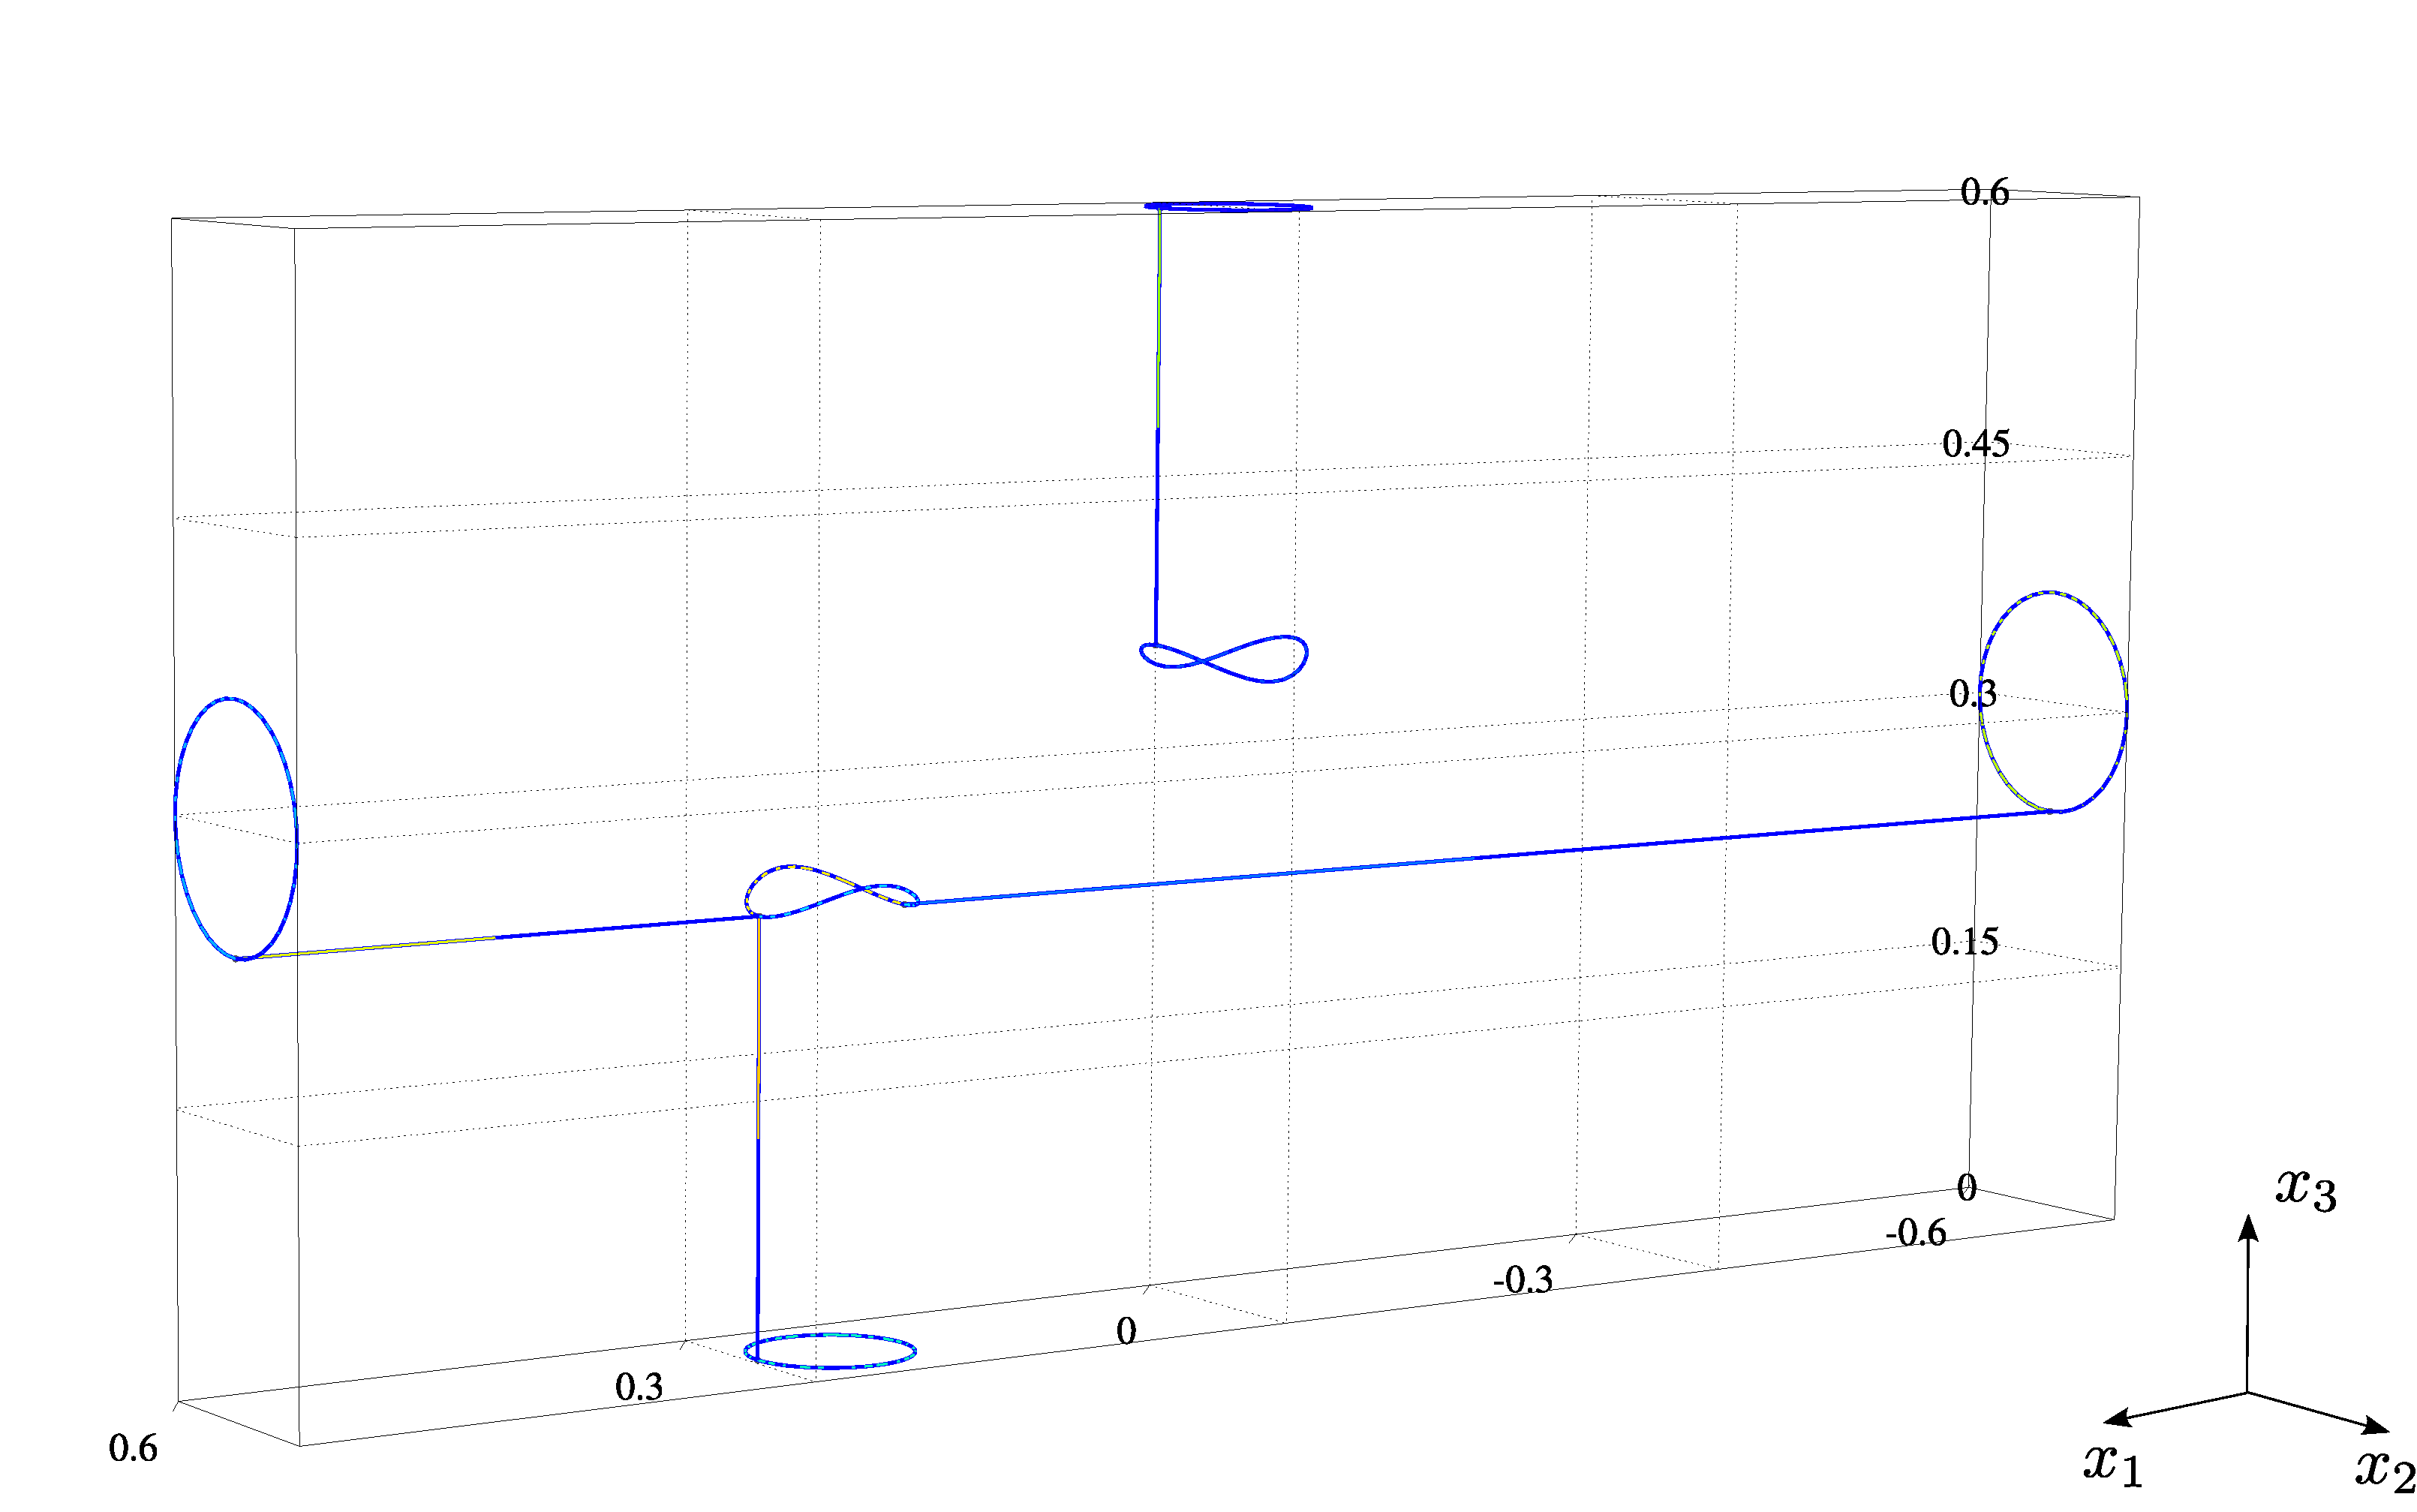
\includegraphics[width=.99\textwidth]{figures/gmsh.pdf}
	\vspace{4mm}
	\caption{Overview of the \texttt{meshgen} package.}
	\label{fig:gmsh}
\end{figure}



\begin{figure}[H]
	\centering
	\vspace{6mm}
	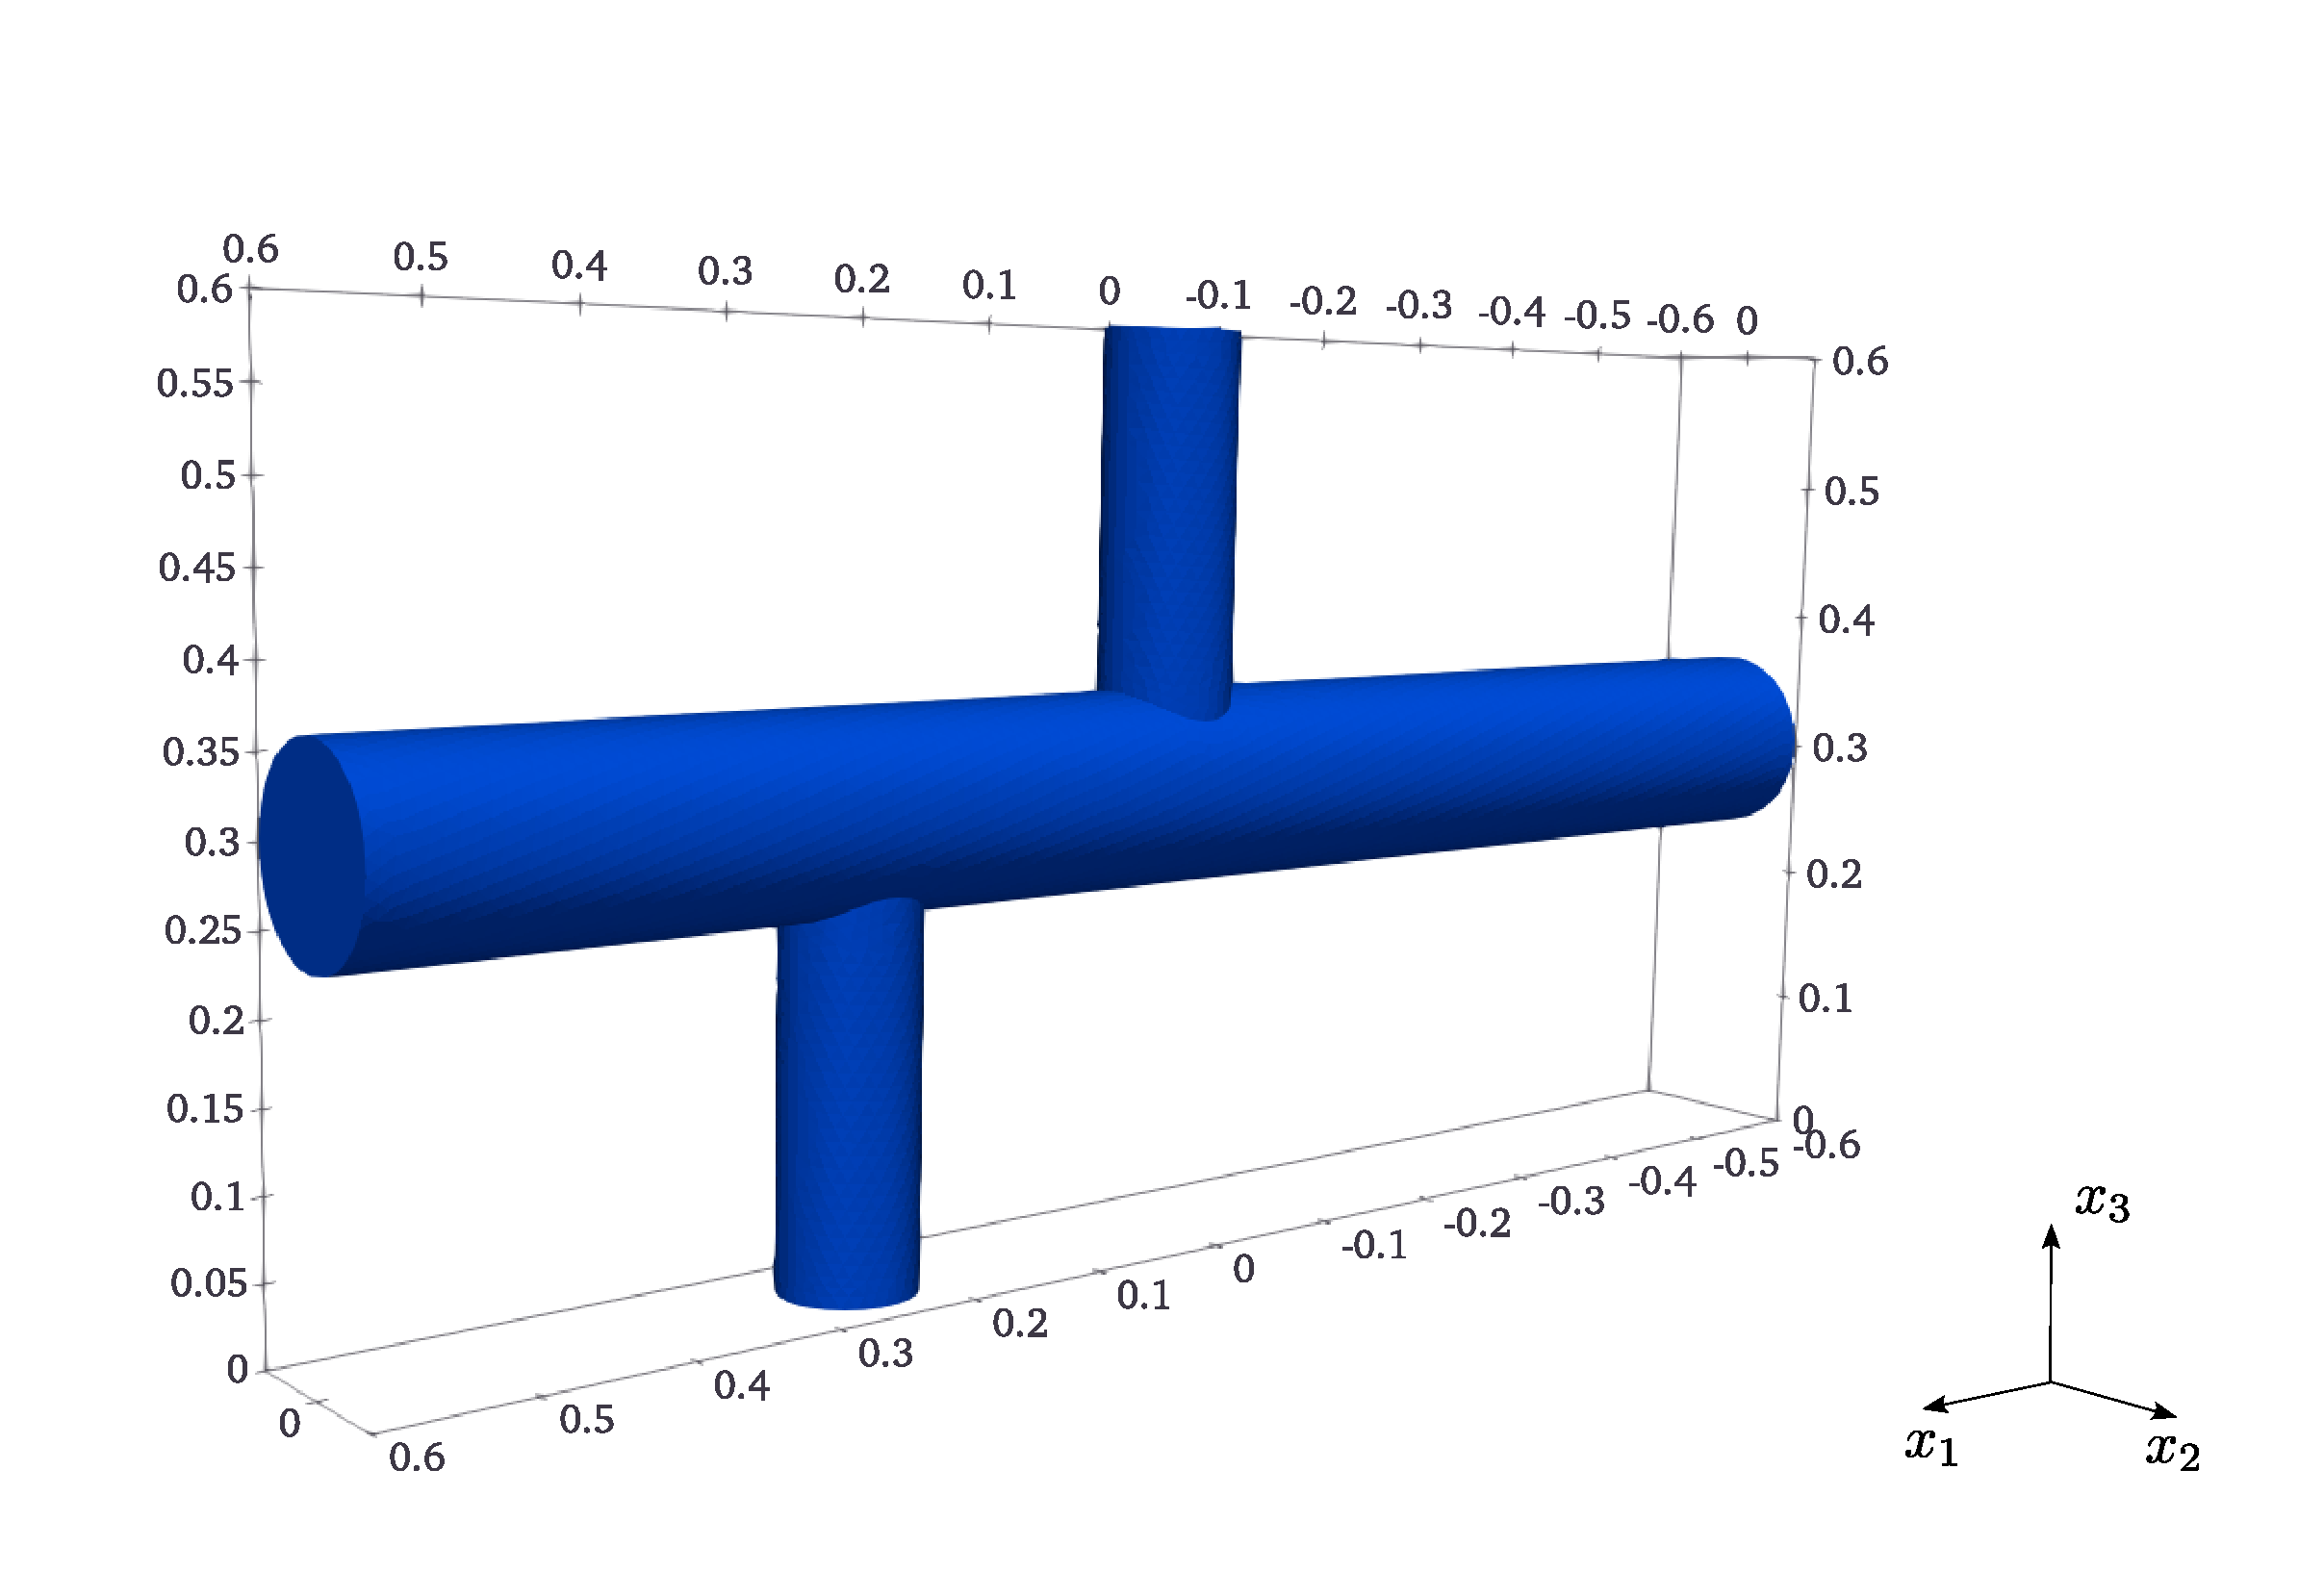
\includegraphics[width=.99\textwidth]{figures/stl.pdf}
	\vspace{4mm}
	\caption{Overview of the \texttt{meshgen} package.}
	\label{fig:stl}
\end{figure}
